%%%%%%%%%%%%%%%%%%%%%%%%%%%%%%%%%%%%%%%%%%%%%%%%%%%%%%%%%%%%%%%%%%%%%%%%% 
% $Id$
% %%%%%%%%%%%%%%%%%%%%%%%%%%%%%%%%%%%%%%%%%%%%%%%%%%%%%%%%%%%%%%%%%%%%%%%%%
%
% Set de slides estudiando diferencias entre uso de Green3D o Green2D
% para problema cilindro infinito usando una seccion (rodaja 3D) del
% cilindro
%
% %%%%%%%%%%%%%%%%%%%%%%%%%%%%%%%%%%%%%%%%%%%%%%%%%%%%%%%%%%%%%%%%%%%%%%%%%

% %%%%%%%%%%%%%%%%%%%%%%%%%%%%%%%%%%%%%%%%%%%%%%%%%%%%%%%%%%%%%%%%%%%%%%%%%
\subsection{Green's Function for 2D Emulation}
% %%%%%%%%%%%%%%%%%%%%%%%%%%%%%%%%%%%%%%%%%%%%%%%%%%%%%%%%%%%%%%%%%%%%%%%%%


\begin{frame}[allowframebreaks]{HOFEM 2D Emulation}

  \begin{columns}
    \column{0.25\textwidth} \centering
    {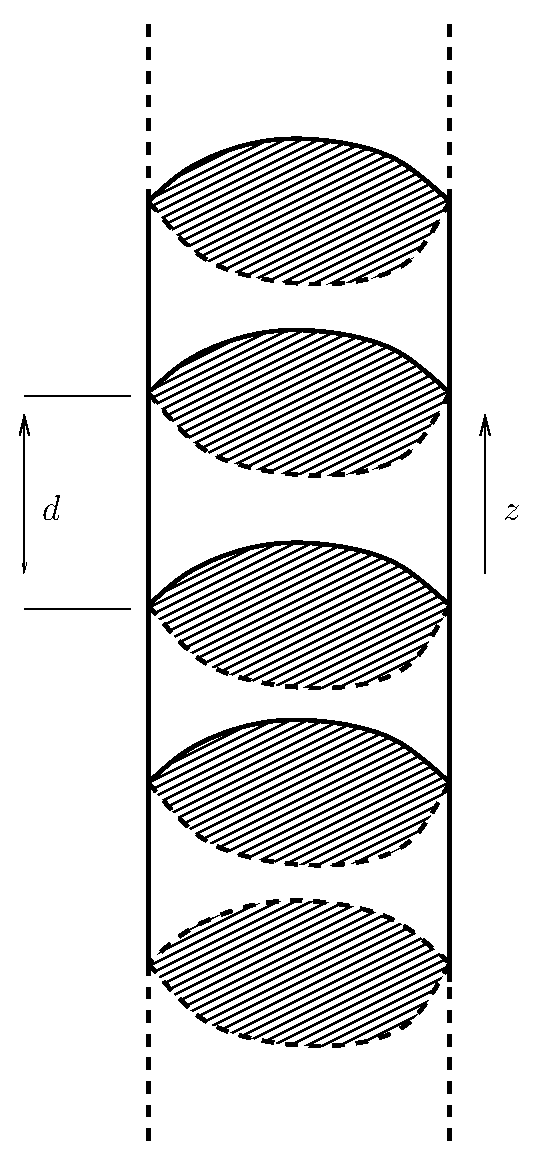
\includegraphics[angle=0,width=\textwidth]{2D_Cylinder_sliced}}

    \column{0.7\textwidth} \centering
    \begin{block}{3D Green's Function}
      \begin{itemize}
      \item Sum of infinite contributions (from each repeated cell)
        
      \item Ewald acceleration needed 
        %
        \begin{equation*}
          \text{Green}(R) = \dfrac{1}{4\pi}
          \sum_{n=-\infty}^\infty \dfrac{e^{-j k R_n}}{R_n}
        \end{equation*}
        with
        \begin{equation*}
          R_n=\abs{\vr-\vrp_n}, \vrp_n=\vrp_0 + n d
        \end{equation*}

        \begin{itemize}
        \item New implementation (for 1D periodicity) required
        \item 1D periodicity case is different (and much more
          involved) than 2D periocicity already present in the code
          for the infinite array.
        \item See details later in Section~\ref{sec:Ewald1D}
        \end{itemize}
      \end{itemize}
      
    \end{block}
  \end{columns}

  \framebreak % %%%%%%%%%%%%%%%%%%%%%%%%%%%%%%%%%%%%%%

  \begin{columns}
    \column{0.25\textwidth} \centering
    {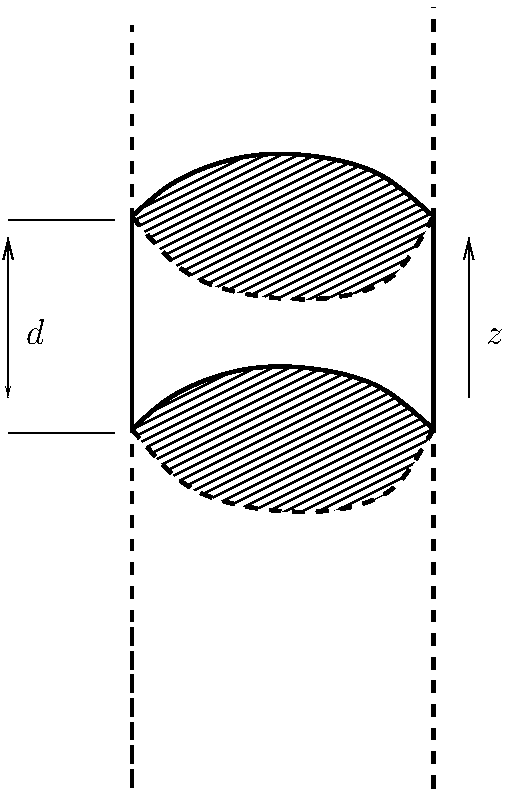
\includegraphics[angle=0,width=\textwidth]{2D_Cylinder_unitslice}}
    
    \column{0.7\textwidth} \centering
    \begin{block}{2D Green's Function}
      \begin{itemize}
      \item No summation needed
        \begin{equation*}
          \text{Green}(\rho) = \dfrac{1}{4\im}  H_0^{(2)}(k|\rho|)
        \end{equation*}
      \end{itemize}
    \end{block}
  \end{columns}

  
 \end{frame}
  

% %%%%%%%%%%%%%%%%%%%%%%%%%%%%%%%%%%%%%%%%%%%%%%%%%%%%%%%%%%%%%%%%%%%%%%%%%
\subsection{Near Field (FE-IIEE loop)}
% %%%%%%%%%%%%%%%%%%%%%%%%%%%%%%%%%%%%%%%%%%%%%%%%%%%%%%%%%%%%%%%%%%%%%%%%%

% %%%%%%%%%%%%%%%%%%%%%%%%%%%%%%%%%%%%%%%%%%%%%%%%%%%%%%%%%%%%%%%

\begin{frame}[allowframebreaks]{Near Field (FE-IIEE loop)}
  
  \begin{block}{Sanity Checks (MATLAB)}
    \begin{itemize}
    \item Equivalence of infinite sum of 3D Green's function with 2D
      Green's function on the unit cell 
  \end{itemize}
    \begin{columns}%[T]
      \column{0.48\textwidth}
      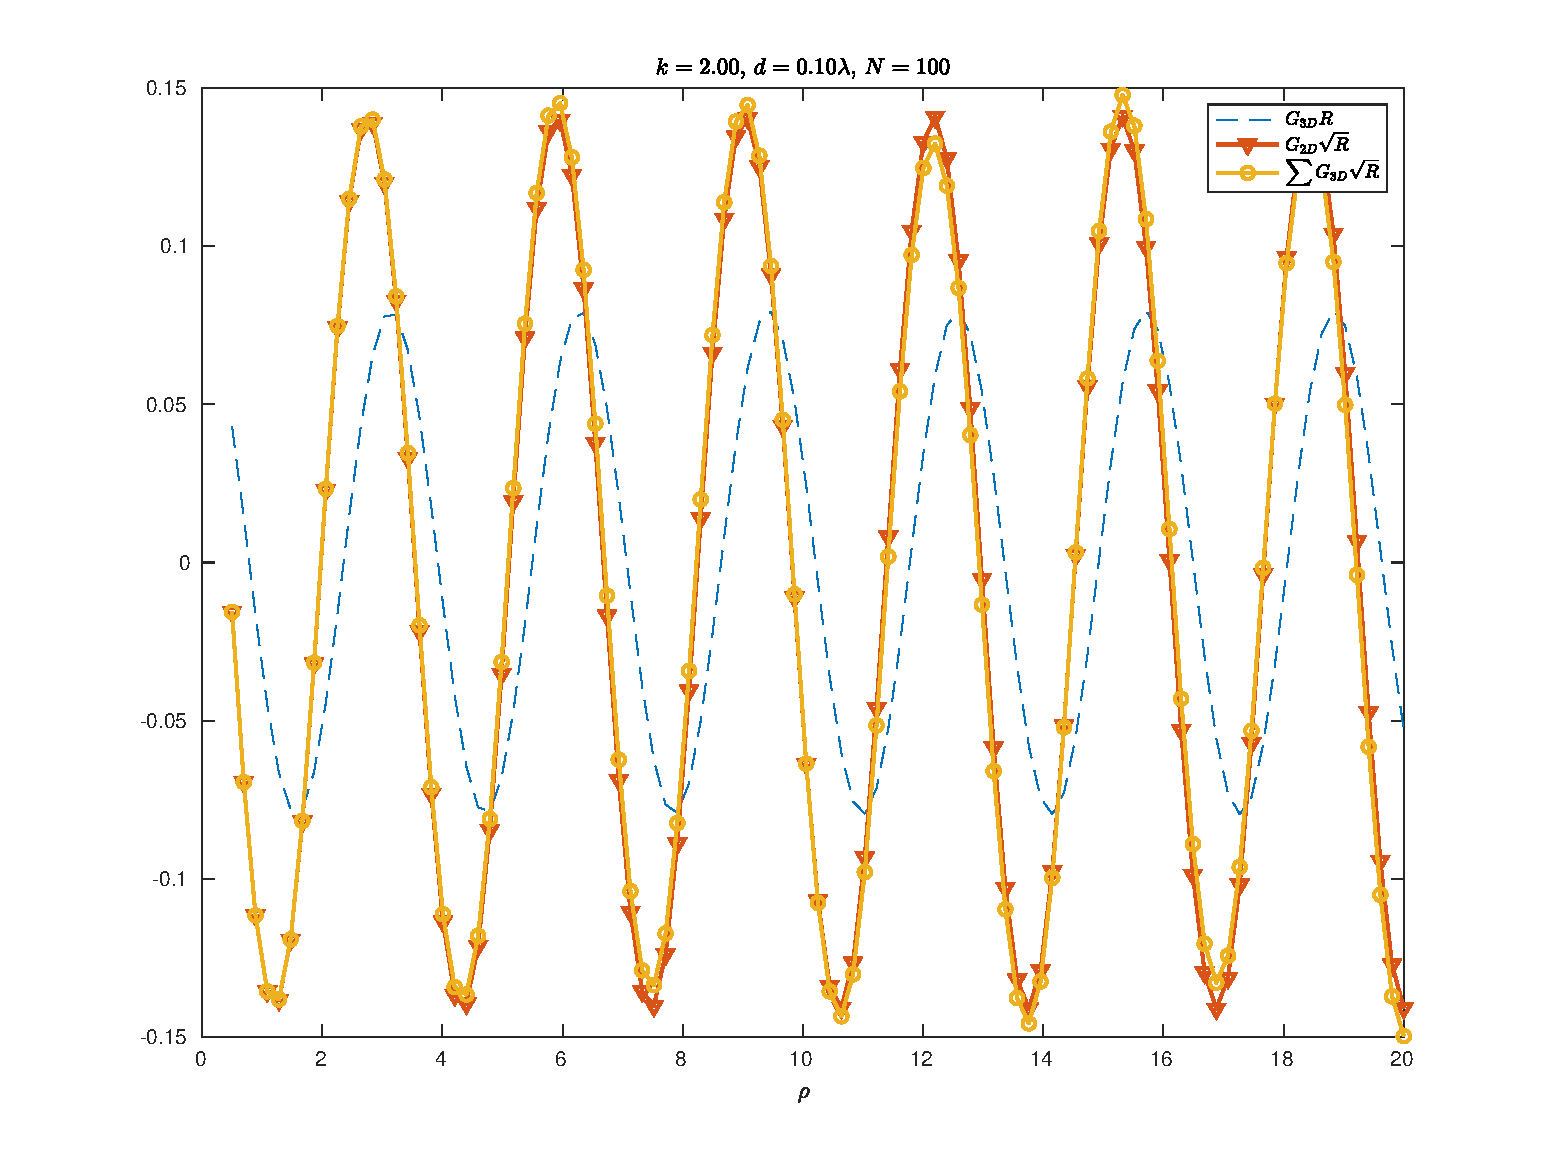
\includegraphics[width=\textwidth]{GreenFunctions_R.pdf} \\
     % \footnotesize{Green's function values as a function of $\rho$}
      \column{0.48\textwidth}
      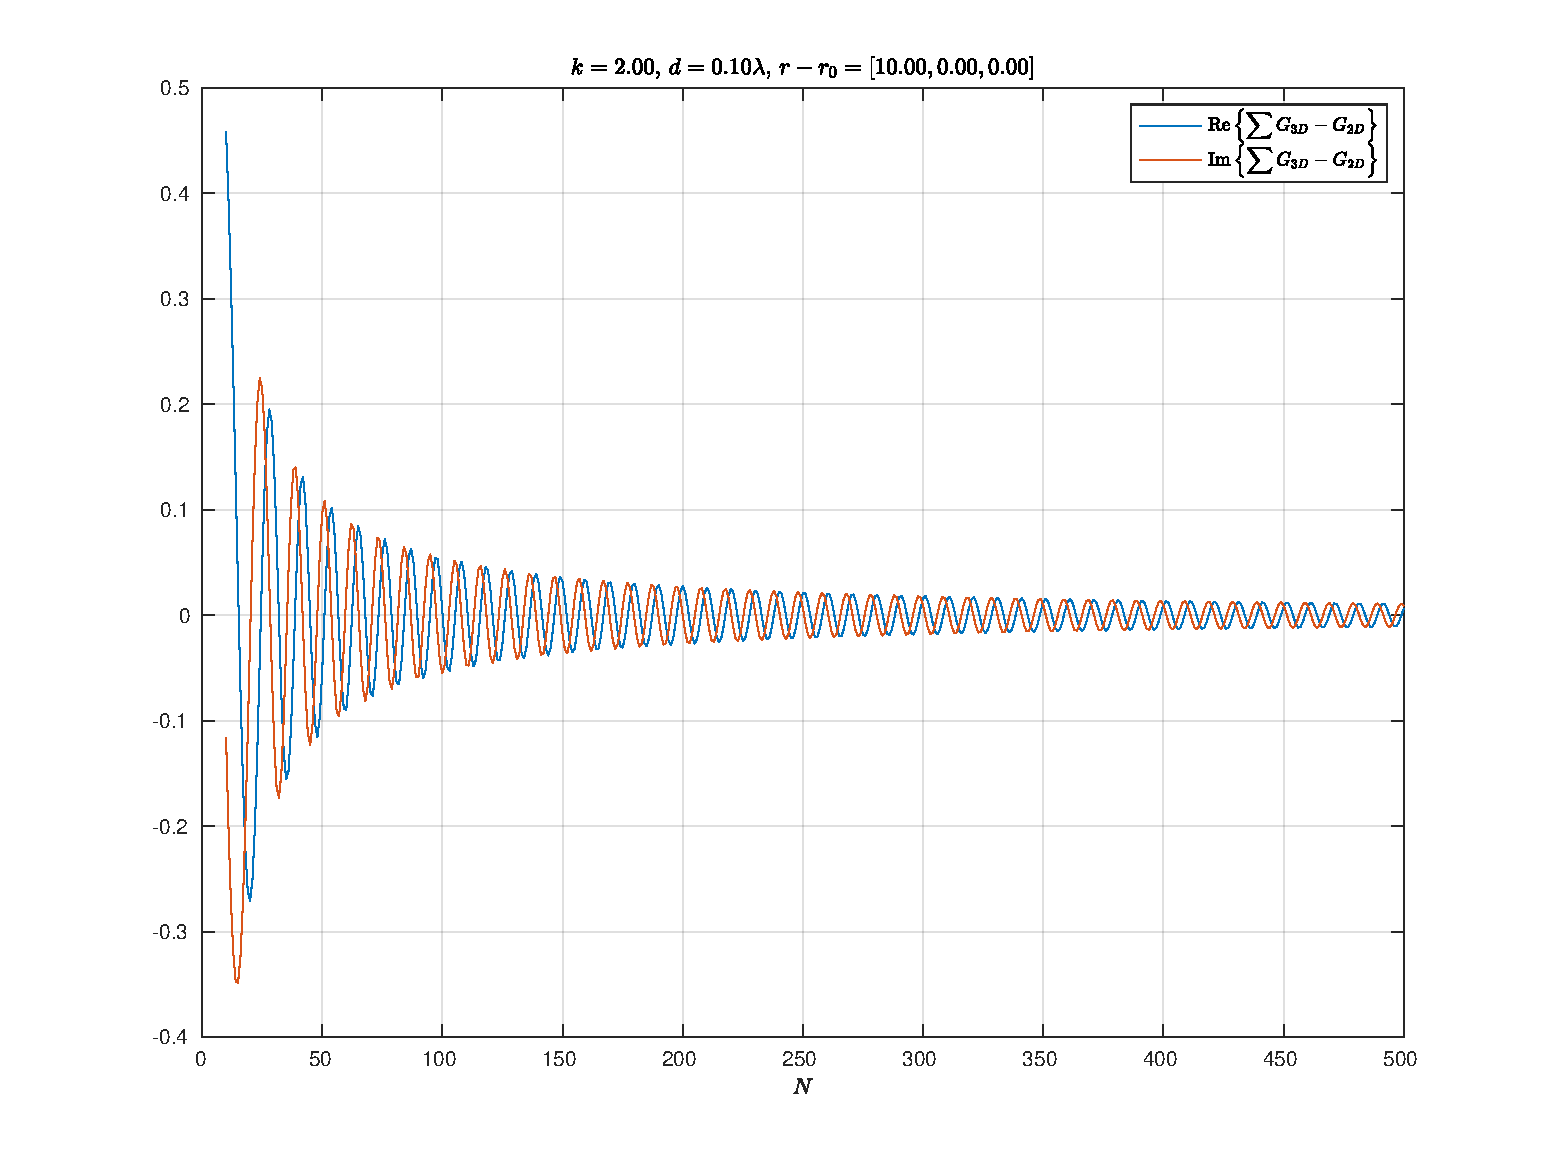
\includegraphics[width=\textwidth]{GreenFunctions_convN_reim.pdf} \\
      %\footnotesize{3D Green's function values as the number of unit
      %  cells considered (no Ewald acceleration)}
    \end{columns}
  \end{block}

  \framebreak % %%%%%%%%%%%%%%%%%%%%%%%%%%%%%%%%%%%%%%

  \begin{block}{Sanity Checks (MATLAB)}
    Equivalence of infinite sum of 3D Green's function with 2D Green's
    function on the unit cell
    \begin{columns}%[T]
      \column{0.48\textwidth}
       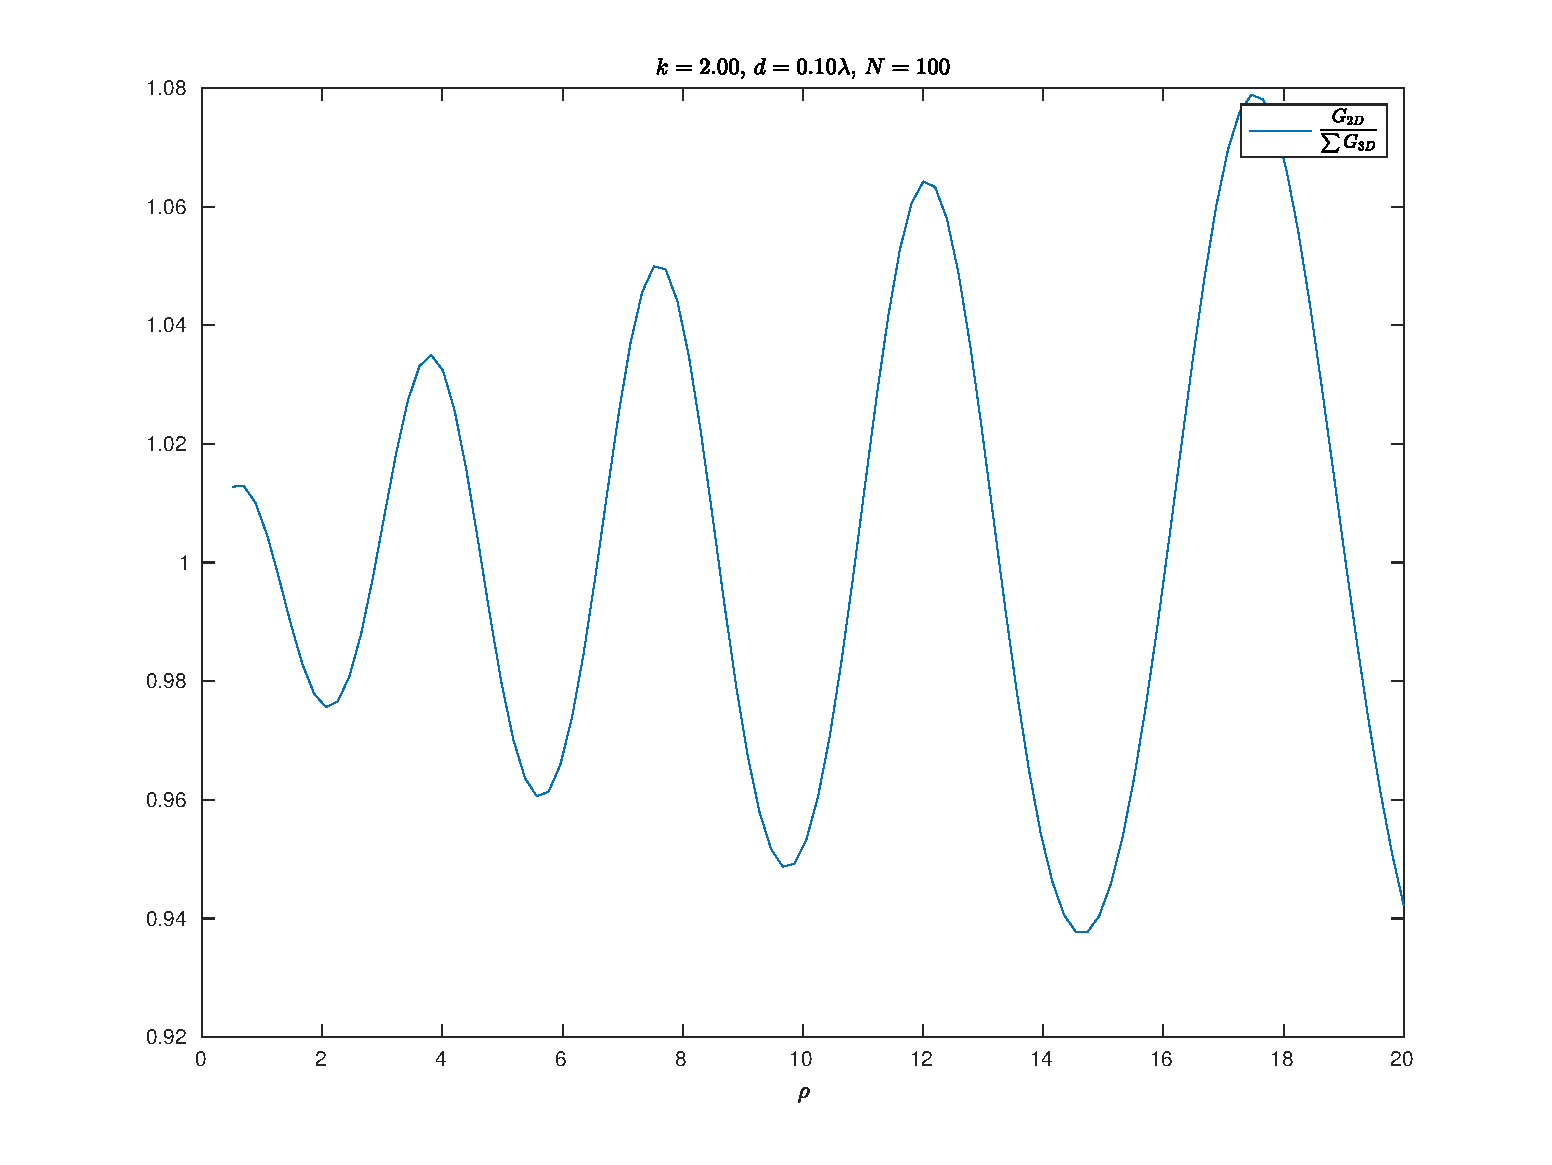
\includegraphics[width=\textwidth]{GreenFunctions_Comp.pdf} \\
%      \footnotesize{Difference Green's function values (3D summation and 2D)
%        as a function of $\rho$}
      \column{0.48\textwidth}
      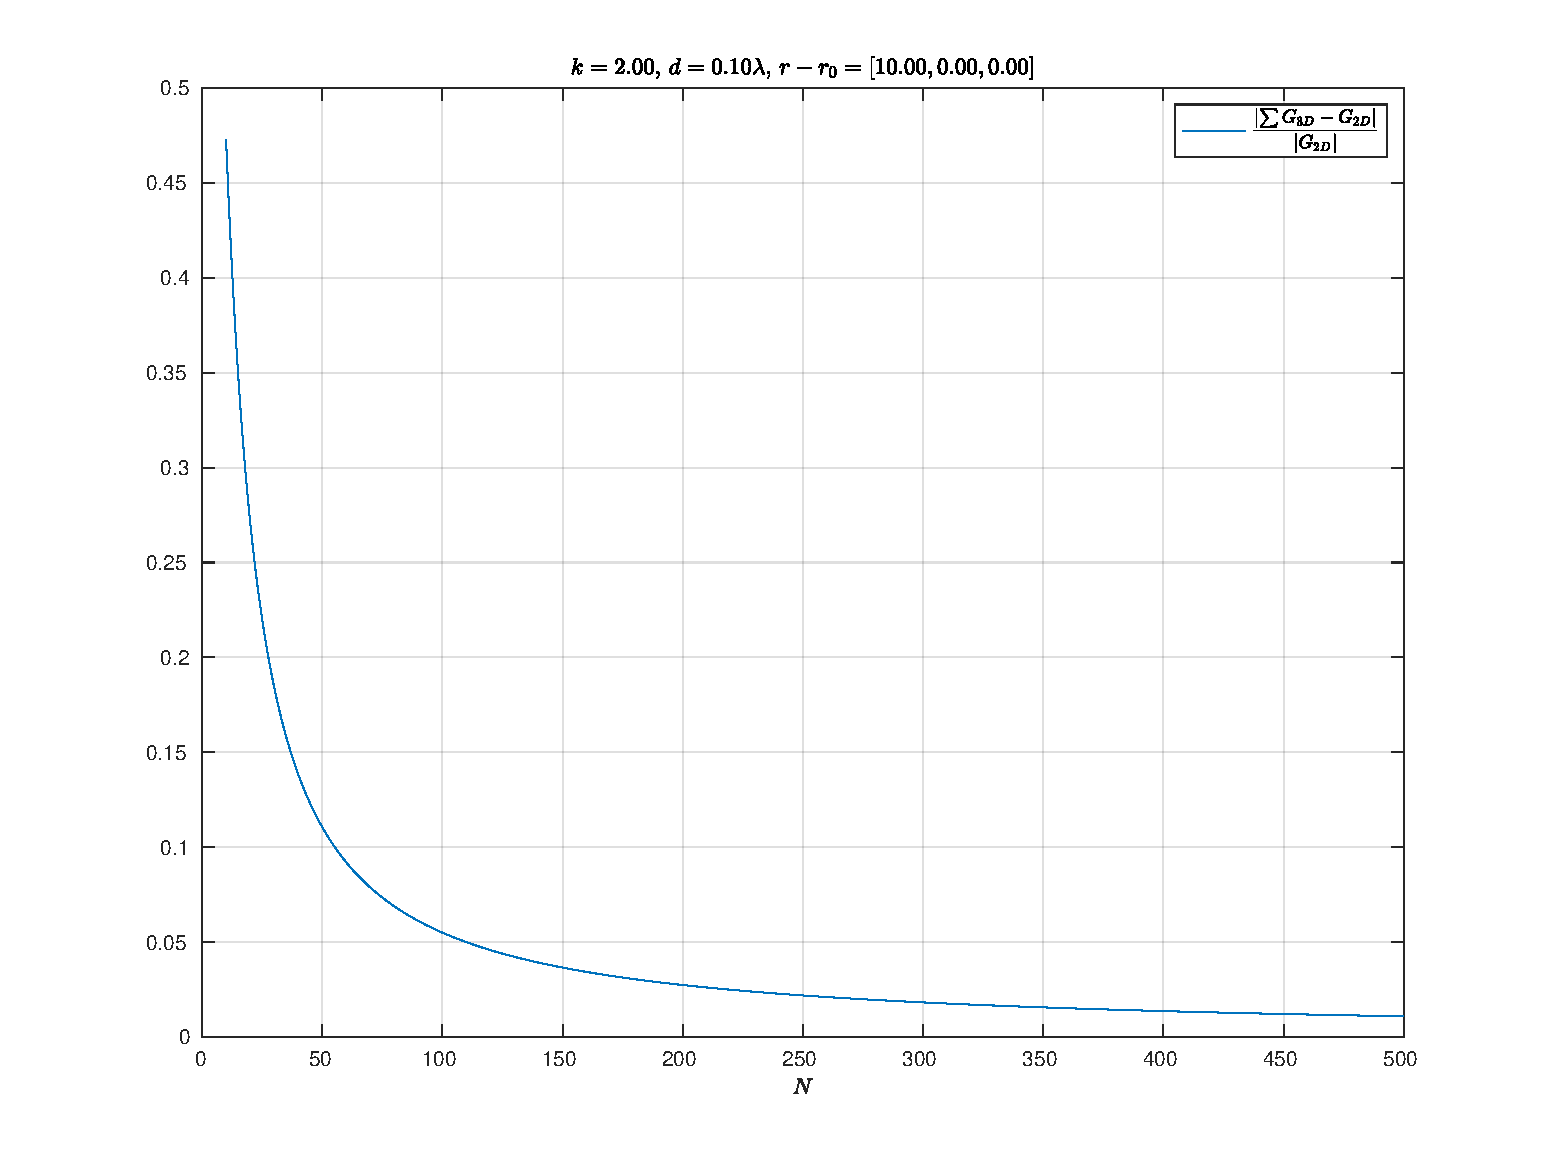
\includegraphics[width=\textwidth]{GreenFunctions_convN_abs.pdf} \\
%      \footnotesize{Difference Green's function values (3D summation
%        and 2D) with the number of unit cells (slices) considered (no
%        Ewald acceleration)}
    \end{columns}
  \end{block}

  \framebreak % %%%%%%%%%%%%%%%%%%%%%%%%%%%%%%%%%%%%%%

  \begin{block}{HOFEM Implementation}

    \begin{itemize}
    \item Coded
    \item Tested
    \end{itemize}
    
    \begin{columns}%[T]
      \column{0.45\textwidth}
      \lstinputlisting[basicstyle=\tiny,tabsize=3,frame=none,
      % caption={3D Green's Function},
      firstline=125,lastline=145]{HOFEM_output_3D_greens_function.txt}
      
      % \column{0.45\textwidth}
      % \lstinputlisting[basicstyle=\tiny,tabsize=3,frame=none,caption={2D
      %   Green's Function},firstline=125,lastline=130]{HOFEM_output_2D_greens_function.txt}
      
    \end{columns}
  \end{block}

  % \framebreak % %%%%%%%%%%%%%%%%%%%%%%%%%%%%%%%%%%%%%%

  % \lstinputlisting[basicstyle=\tiny,tabsize=3,frame=none,caption={2D
  %   Green's Function},firstline=20,lastline=30]{HOFEM_output_diff_3D_2D_greens_function_sidebyside.txt}

  \framebreak % %%%%%%%%%%%%%%%%%%%%%%%%%%%%%%%%%%%%%%

 Code output (terminal):
  
 \lstinputlisting[basicstyle=\scriptsize,tabsize=3,frame=none,
 % caption={2D Green's Function}
 ]{HOFEM_output_diff_3D_2D_greens_function_iterations.txt}


  \framebreak % %%%%%%%%%%%%%%%%%%%%%%%%%%%%%%%%%%%%%%


  \begin{columns}
    \column{0.48\textwidth} \centering
    {\includegraphics[angle=0,width=\textwidth]{Cylinder_0_5b_nearfield_3D_greens}}
    \column{0.48\textwidth} \centering
    {\includegraphics[angle=0,width=\textwidth]{Cylinder_0_5b_nearfield_3D_greens}}
  \end{columns}    

  
\end{frame}


% %%%%%%%%%%%%%%%%%%%%%%%%%%%%%%%%%%%%%%%%%%%%%%%%%%%%%%%%%%%%%%%%%%%%%%%%%
\subsection{Far Field (postprocess)}
% %%%%%%%%%%%%%%%%%%%%%%%%%%%%%%%%%%%%%%%%%%%%%%%%%%%%%%%%%%%%%%%%%%%%%%%%%

\begin{frame}[allowframebreaks]{Far Field (postprocess)}

  \begin{block}{Equivalence of Green's Functions for Far Field}
    \begin{itemize}
    \item Can we use an infinite sum of 3D Green's far-field functions
      to model the 2D Green's far-field?
      \begin{itemize}
      \item \alert {NO}
      \item and it makes sense!
      \end{itemize}
    \end{itemize}
  \end{block}
    

  \begin{block}{Far Field as Fourier Transform} 
      The Fourier Transform of a constant current contribution along
      $z$ is a delta function in the spatial frequency domain, i.e.,
      variable $\theta$:
      % 
      \begin{equation}
        \text{Far Field}(\theta,\phi) =  \alert{\delta(\theta-\pi/2)}  F(\phi)
      \end{equation}
      
    \end{block}
  
    \framebreak % %%%%%%%%%%%%%%%%%%%%%%%%%%%%%%%%%%%%%%

    \begin{columns}
      \column{0.46\textwidth} \centering
      \begin{block}{$\theta\ne 90^\circ$: \alert{Oscillations}}
        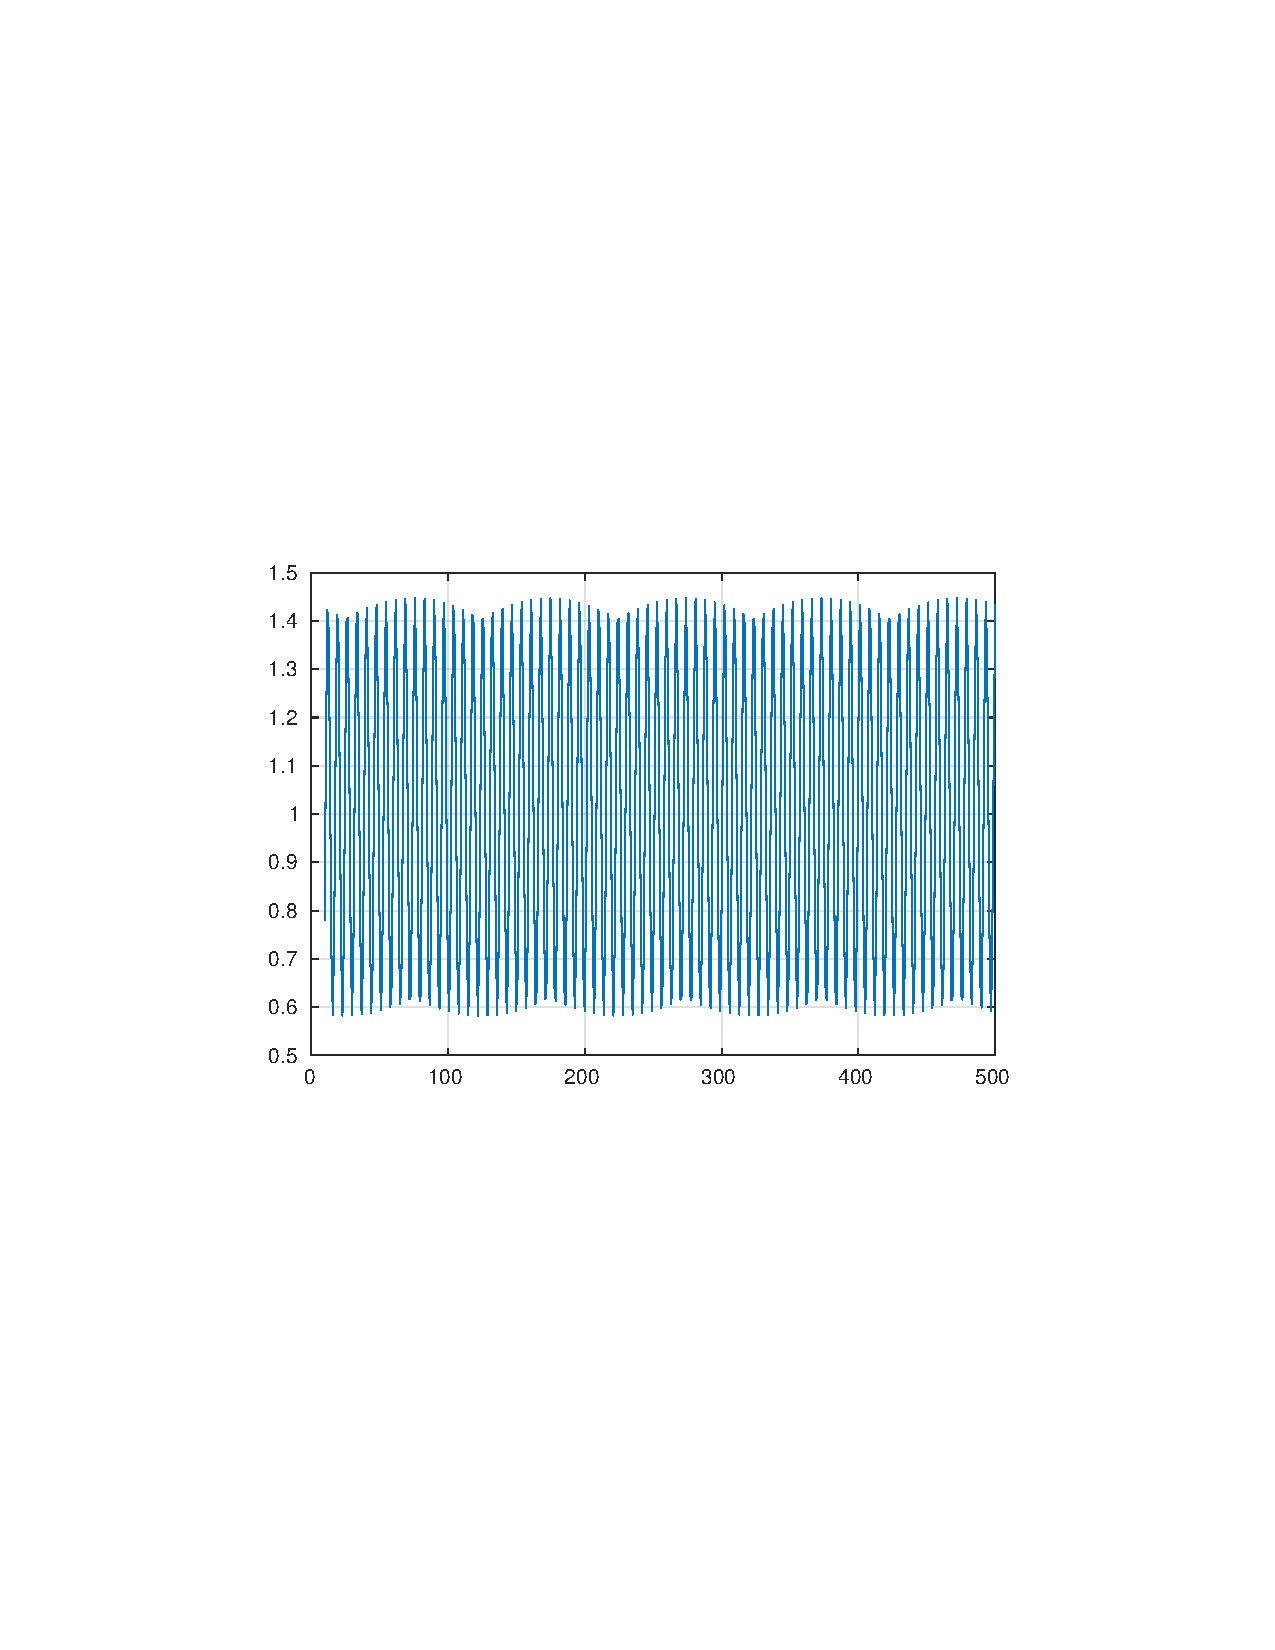
\includegraphics[clip=true,trim=100 200 100 200,width=\textwidth]{GreenFar_abs_theta45} \\
      \end{block}
      
      \column{0.46\textwidth} \centering
      \begin{block}{$\theta=90^\circ$: \alert{Divergence}}
        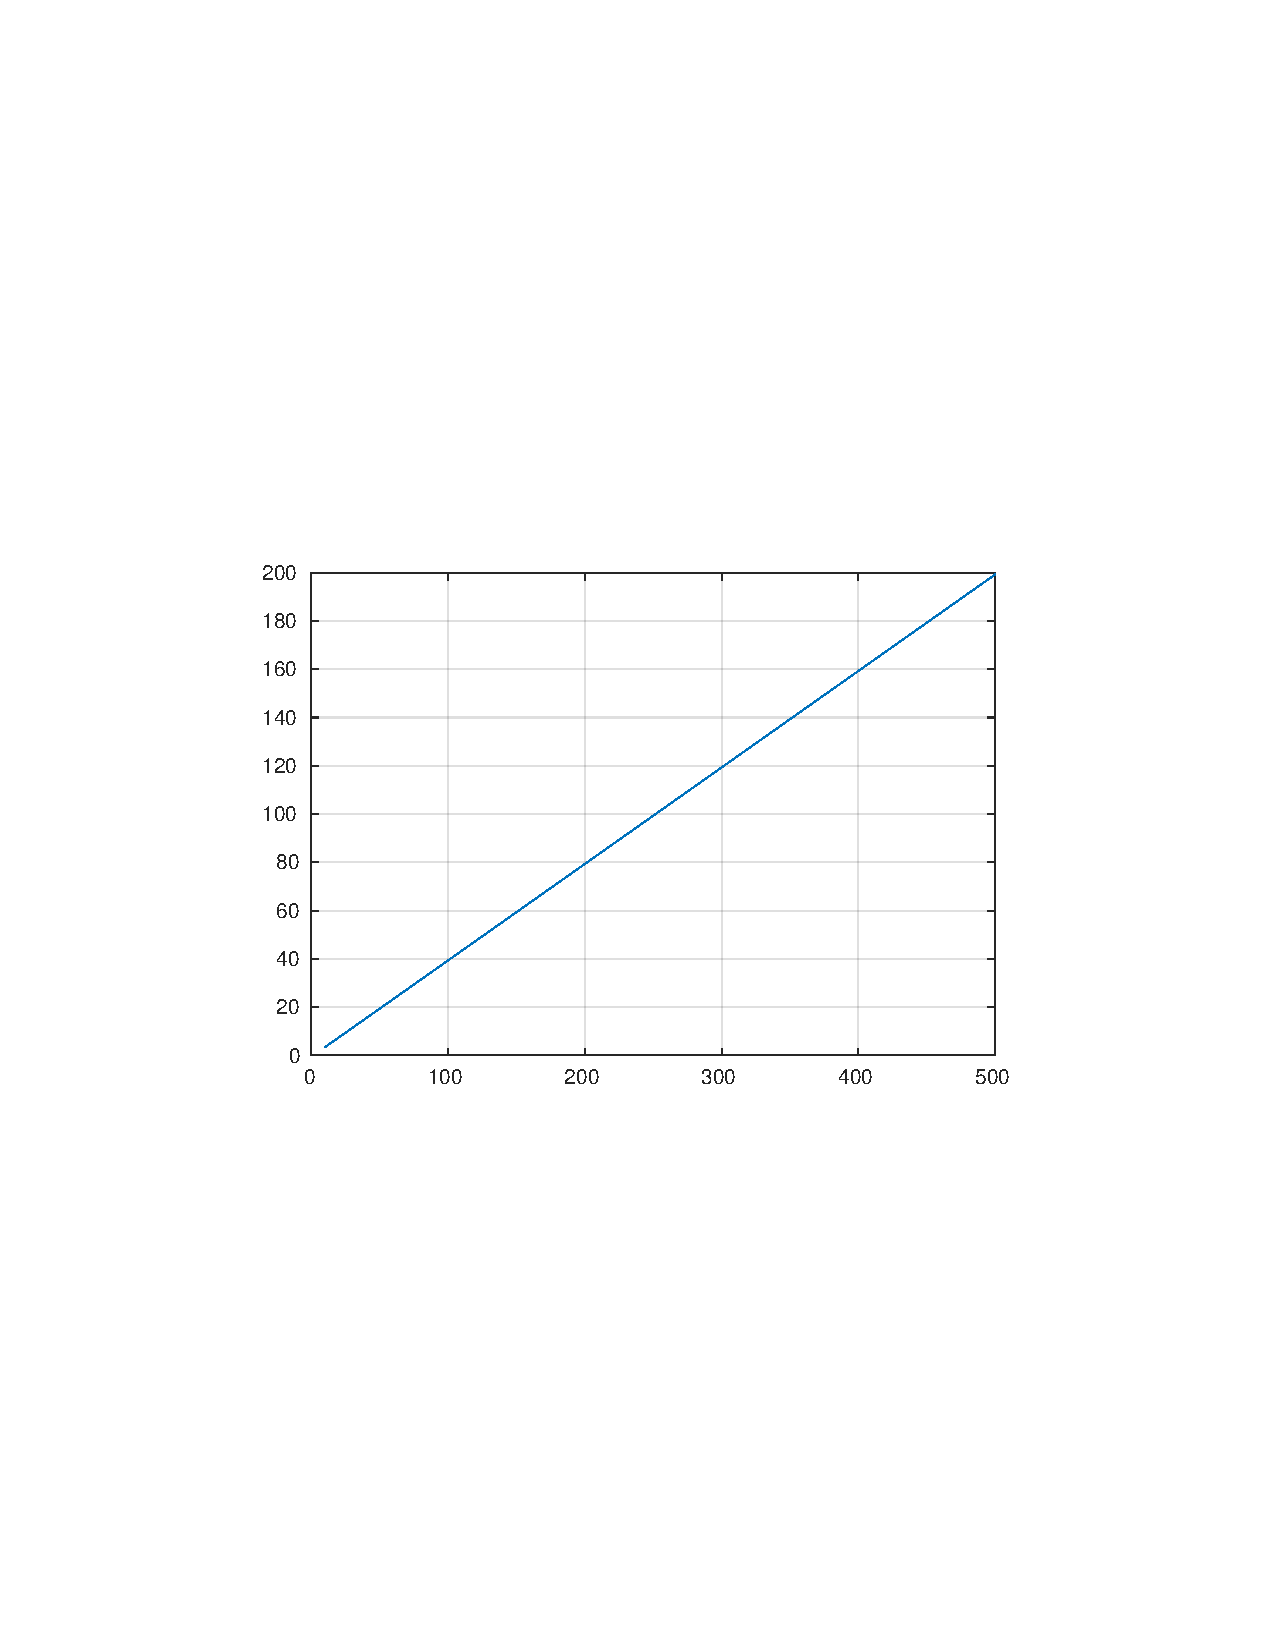
\includegraphics[clip=true,trim=100 200 100 200,width=\textwidth]{GreenFar_abs_theta90} \\
      \end{block}
            
    \end{columns}

  \end{frame}
  
  % %%%%%%%%%%%%%%%%%%%%%%%%%%%%%%%%%%%%%%%%%%%%%%%%%%%%%%%%%%%%%%%

% %%%%%%%%%%%%%%%%%%%%%%%%%%%%%%%%%%%%%%%%%%%%%%%%%%%%%%%%%%%%%%%%%%%%%%%%%
\subsection{Further Rethinking on Possible Use of  {\GreenT}}
% %%%%%%%%%%%%%%%%%%%%%%%%%%%%%%%%%%%%%%%%%%%%%%%%%%%%%%%%%%%%%%%%%%%%%%%%%

    
  \begin{frame}[plain]
    \centering    \Large{Rethinking\ldots}

    \vspace*{0.5\baselineskip}

    \centering\parbox{\textwidth}{%
      AIRBUS: \emph{\foreignlanguage{spanish}{hay un chico con nosotros que
          resuelve problemas de scattering de cilindros y no usa
          función de Hankel. Usa Green3D para calcular el campo
          (lejano) de scattering de una rodaja y \alert{le funciona.}}
        }}

      \vspace*{\baselineskip}
      
      \begin{itemize}
      \item Further study of differences between  {\GreenD} and {\GreenT}
        \begin{itemize}
        \item Obvious (after a maturation process) for far field
        \item Not so obvious for near field (i.e., in its impact in
          FE-IIEE loop)
        \end{itemize}
      \end{itemize}
      
  \end{frame}
  

% %%%%%%%%%%%%%%%%%%%%%%%%%%%%%%%%%%%%%%%%%%%%%%%%%%%%%%%%%%%%%%%

\begin{frame}[allowframebreaks]{Far Field (postprocess)}

  \begin{block}{Equivalence of Green's Functions for Far Field}
    \begin{itemize}
    \item Can we use an infinite sum of 3D Green's far-field functions
      to model the 2D Green's far-field?
      \begin{itemize}
      \item NO
      \item and it makes sense!
      \item No need of infinite sum (\alert{far field {\GreenT}/{\GreenD} is enough})
        \begin{itemize}
        \item Note that far field versions of {\GreenT} (with
          $r=\rho$) and {\GreenD} are equal up to a constant
        \end{itemize}

      \end{itemize}
    \end{itemize}
  \end{block}
    

  \begin{block}{Far Field as Fourier Transform} 
      The Fourier Transform of a constant current contribution along
      $z$ is a delta function in the spatial frequency domain, i.e.,
      variable $\theta$:
      % 
      \begin{equation}
        \text{Far Field}(\theta,\phi) =  \alert{\delta(\theta-\pi/2)}  F(\phi)
      \end{equation}
      
    \end{block}
  
    \framebreak % %%%%%%%%%%%%%%%%%%%%%%%%%%%%%%%%%%%%%%
    
    \begin{block}{{\GreenD} vs {\GreenT}}

      
      $F(\phi)$ is the same (after normalization) considering asymptotic
      expressions of {\GreenT} and {\GreenT}
      
    \begin{columns}\centering
      \column{0.4\textwidth}% \centering
      %
      \begin{equation*}
        H_0^{(2)}(k\rho)
        \enskip \overset{\rho\rightarrow\infty}{\approx} \enskip
        \sqrt{\dfrac{2 j }{\pi k \rho}} \, e^{-jk\rho}
      \end{equation*}

      \column{0.4\textwidth}% \centering
      % 
      % 
      \begin{equation*}
        \dfrac{e^{-jkR}}{4\pi R}
         \enskip \overset{r\rightarrow\infty}{\approx}  \enskip
        \dfrac{e^{-jkr}}{4\pi r} e^{j k r^\prime\! \cos\psi}
      \end{equation*}

    \end{columns}
    
    \end{block}


  \end{frame}

  
% %%%%%%%%%%%%%%%%%%%%%%%%%%%%%%%%%%%%%%%%%%%%%%%%%%%%%%%%%%%%%%%

\begin{frame}[allowframebreaks]{Near Field (FE-IIEE loop)}
  
% {\Gree3D vs {\GreenD} }


 Code output (terminal):

 \begin{itemize}
 \item From previous meeting % Large $S'-S$
   \begin{columns}%[T]
   \column{0.45\textwidth} {\GreenD} 
   \column{0.45\textwidth} {\GreenT} 
 \end{columns}   

 \lstinputlisting[basicstyle=\scriptsize,tabsize=3,frame=none,
 % caption={2D Green's Function}
 ]{HOFEM_output_diff_3D_2D_greens_function_iterations_reversed.txt}

 \vspace{\baselineskip}

 \alert{How can it work?} Note we used {\GreenT} itself (only one
 slide was considered)
 
 
 \framebreak % %%%%%%%%%%%%%%%%%%%%%%%%%%%%%%%%%%%%%%

 Code output (terminal):

 \item Large $S'-S$
   \begin{columns}[T]
   \column{0.45\textwidth} {\GreenD} 
   \column{0.45\textwidth} {\GreenT} 
 \end{columns}   

 \lstinputlisting[basicstyle=\scriptsize,tabsize=3,frame=none,
 ]{HOFEM_output_diff_3D_2D_greens_function_iterations_reversed.txt}
 
\item Small $S'-S$
   \begin{columns}%[T]
   \column{0.45\textwidth} {\GreenD} 
   \column{0.45\textwidth} {\GreenT} 
 \end{columns}   

 \lstinputlisting[basicstyle=\scriptsize,tabsize=3,frame=none,
 ]{HOFEM_output_diff_3D_2D_greens_function__small_S-Sp_iterations_reversed.txt}

 
\end{itemize}

\end{frame}

  % %%%%%%%%%%%%%%%%%%%%%%%%%%%%%%%%%%%%%%%%%%%%%%%%%%%%%%%%%%%%%%% 

% \begin{frame}[allowframebreaks]{Study of {\GreenT} vs {\GreenD}}
 
 
%   \textbf{GRAFICAS DE LAS GEOMETRIAS USADAS EN LAS PRUEBAS}


%   \begin{itemize}
%   \item Lo que le enseñamos meeting pasado fue sobre (S'-S grande,
%     espesor pequeño y S,S' rectangulares):
    
% \begin{verbatim}
% |`cylinder_05b_1`               |1      |1      |0.05     |Rectangular    |Rectangular      |1
% \end{verbatim}
    
%     \item Durante el finde (S'-S pequeño y espesor grande, con S', S circulares)
  
% \begin{verbatim}
%     |`cylinder_05e_01_01_075`       |0.1    |0.1    |1        |Circular       |Circular         |0.75
% \end{verbatim}

%     \item Para ver efecto del espesor se puede comparar 
      
% \begin{verbatim}
%     |`cylinder_05e_01_01_075`       |0.1    |0.1    |1        |Circular       |Circular         |0.75
%     |`cylinder_sp_circled_s_circled_d_1_h_005_m_075`  |0.1|0.1|0.05   |Circular    |Circular     |0.75
% \end{verbatim}

%     \item Mallado con S' sobre PEC para paranoias de J,M equivalentes.

%       Uno de los:
% \begin{verbatim}
% Espesor bajo, distancia S-S' baja:
% |`cylinder_sp_pec_s_circled_d_01_h_005_m_07`  |0  |0.1|0.05   |Circular |Circular     |0.7


% Espesor alto, distancia S-S' baja:
% |`cylinder_sp_pec_s_circled_d_01_h_1_m_07`    |0  |0.1|1      |Circular |Circular     |0.7
% \end{verbatim}

      
      
%   \end{itemize}
% \end{frame}

  % %%%%%%%%%%%%%%%%%%%%%%%%%%%%%%%%%%%%%%%%%%%%%%%%%%%%%%%%%%%%%%% 

\begin{frame}[allowframebreaks]{{\GreenD} vs {\GreenT}}{Comparison
    with analytical solution}

  \begin{itemize}
  \item Most results displayed correspond to TM and E field
  \item H field (i.e., RotE) identical conclusions
  \item By duality (satisfied by HOFEM) TE results ``should'' be
    identical (tested).
  \item Most results shown here correspond to both $S'$ and $S$
    conformal to the cylinder (circular boundary). Analogous
    results/conclusions are obtained with rectangular boundaries for
    $S'$ and $S$ (and combinations of them).
  \end{itemize}
  % \textbf{\url{cylinder_05e_01_01_075} ¿Graficas del estilo de??}

  \framebreak % %%%%%%%%%%%%%%%%%%%%%%%%%%%%

  
    \begin{columns}
        \column{0.55\textwidth}
    \includegraphics[width=\linewidth]
    {results/2D/20/300/\meshCCC{01}{1}{075}/geometry.pdf}
        \column{0.4\textwidth}
        \begin{itemize}
          \item 300\,MHz
          \item Small $S-S'$
          \item Thick slice
        \end{itemize}
    \end{columns}

    \framebreak

    Evolution scattered electric field ($S'$ over $S$)

    \vbs

    Iteration \makebox[0pt][l]{1:}\hspace{2em}
    \raisebox{\baselineskip-\height}{
      \includegraphics[width=0.3\textwidth]
      {results/2D/1/300/\meshCCC{01}{1}{075}/E_S.pdf}
      \hspace{1cm}
      \includegraphics[width=0.3\textwidth]
      {results/3D/1/300/\meshCCC{01}{1}{075}/E_S.pdf}
    }

    \vbs

    Iteration \makebox[0pt][l]{20:}\hspace{2em}
    \raisebox{\baselineskip-\height}{
      \includegraphics[width=0.3\textwidth]
      {results/2D/20/300/\meshCCC{01}{1}{075}/E_S.pdf}
      \hspace{1cm}
      \includegraphics[width=0.3\textwidth]
      {results/3D/20/300/\meshCCC{01}{1}{075}/E_S.pdf}
    }

    
    \framebreak
    Evolution scattered magnetic field ($S'$ over $S$)

    \vbs

    Iteration \makebox[0pt][l]{1:}\hspace{2em}
    \raisebox{\baselineskip-\height}{
      \includegraphics[width=0.3\textwidth]
      {results/2D/1/300/\meshCCC{01}{1}{075}/H_S.pdf}
      \hspace{1cm}
      \includegraphics[width=0.3\textwidth]
      {results/3D/1/300/\meshCCC{01}{1}{075}/H_S.pdf}
    }

    \vbs

    Iteration \makebox[0pt][l]{20:}\hspace{2em}
    \raisebox{\baselineskip-\height}{
      \includegraphics[width=0.3\textwidth]
      {results/2D/20/300/\meshCCC{01}{1}{075}/H_S.pdf}
      \hspace{1cm}
      \includegraphics[width=0.3\textwidth]
      {results/3D/20/300/\meshCCC{01}{1}{075}/H_S.pdf}
    }


    \framebreak

    Evolution electric field on $S'$

    \vbs

    Iteration \makebox[0pt][l]{1:}\hspace{2em}
    \raisebox{\baselineskip-\height}{
      \includegraphics[width=0.3\textwidth]
      {results/2D/1/300/\meshCCC{01}{1}{075}/E_Sp.pdf}
      \hspace{1cm}
      \includegraphics[width=0.3\textwidth]
      {results/3D/1/300/\meshCCC{01}{1}{075}/E_Sp.pdf}
    }

    \vbs

    Iteration \makebox[0pt][l]{20:}\hspace{2em}
    \raisebox{\baselineskip-\height}{
      \includegraphics[width=0.3\textwidth]
      {results/2D/20/300/\meshCCC{01}{1}{075}/E_Sp.pdf}
      \hspace{1cm}
      \includegraphics[width=0.3\textwidth]
      {results/3D/20/300/\meshCCC{01}{1}{075}/E_Sp.pdf}
    }

    \framebreak

    \begin{itemize}
    \item Higher error with {\GreenT}
      \begin{itemize}
      \item This is a case with small distance $S-S'$ and large thickness
      \item Nevertheless, the error is always significantly higher
        than {\GreenD}
      \end{itemize}
    \item {\GreenT} does not converge to right solution
    \item Components $E_x$, $E_z$, $H_y$ are not null \\
      \footnotesize{(issue of \alert{($\ast$)} certainly added confusion on the
      debugging/verification of the code)}
      \begin{itemize}
      \item Much higher levels with {\GreenT}
      \item {\GreenT} (the Green's function itself) generates non null
        $E_x$, $E_z$, $H_y$ from $E_z$ on $S'$
      \item {\GreenD} (the Green's function itself) does not generate
        any $E_x$, $E_z$, $H_y$
        \begin{itemize}
        \item Numerically, non-zero levels of $E_x$, $E_z$, $H_y$ are
          generated because numerical FEM solution has non zero levels of
          $E_x$, $E_z$, $H_y$ (tested!)
        \end{itemize}
      \end{itemize}
    \item Numerical noise always present  due to discretization 
      \begin{itemize}
      \item Clearly visible in this case
      \item Decreases with finer discretization ---FEM mesh--- (tested!)
      \end{itemize}
    \end{itemize}
    
    {\footnotesize \alert{($\ast$)} Issue of GiD/HOFEM-GUI representation of fields on surface}
  
\end{frame}

% %%%%%%%%%%%%%%%%%%%%%%%%%%%%%%%%%%%%%%%%%%%%%%%%%%%%%%%%%%%%%%%

% Esto es un tema que no esta relacionado directamente con 2D
% Emulation sino genral del código pero se lo cuento aqui a Airbus
% porque viene a cuento.

% %%%%%%%%%%%%%%%%%%%%%%%%%%%%%%%%%%%%%%%%%%%%%%%%%%%%%%%%%%%%%%%%%%%%%%%%%
\subsection{A note on Field Representation on Surfaces}
% %%%%%%%%%%%%%%%%%%%%%%%%%%%%%%%%%%%%%%%%%%%%%%%%%%%%%%%%%%%%%%%%%%%%%%%%%

\begin{frame}[plain]
  \centering    \Large{Rethinking\ldots}
  
  {\footnotesize \alert{($\ast$)} Issue of GiD/HOFEM-GUI representation of fields on surface}
  
\end{frame}

% %%%%%
  
\begin{frame}[allowframebreaks]{GiD/HOFEM-GUI Field Representation 
    on Surfaces}{Examples with PEC surfaces}

  \begin{itemize}
  \item $E_z$ should be null on the  caps (top and
    bottom $y=\text{cte}$)

    \vbs
   
    \begin{columns}%[T]
      \centering
      \column{0.48\textwidth}\centering
      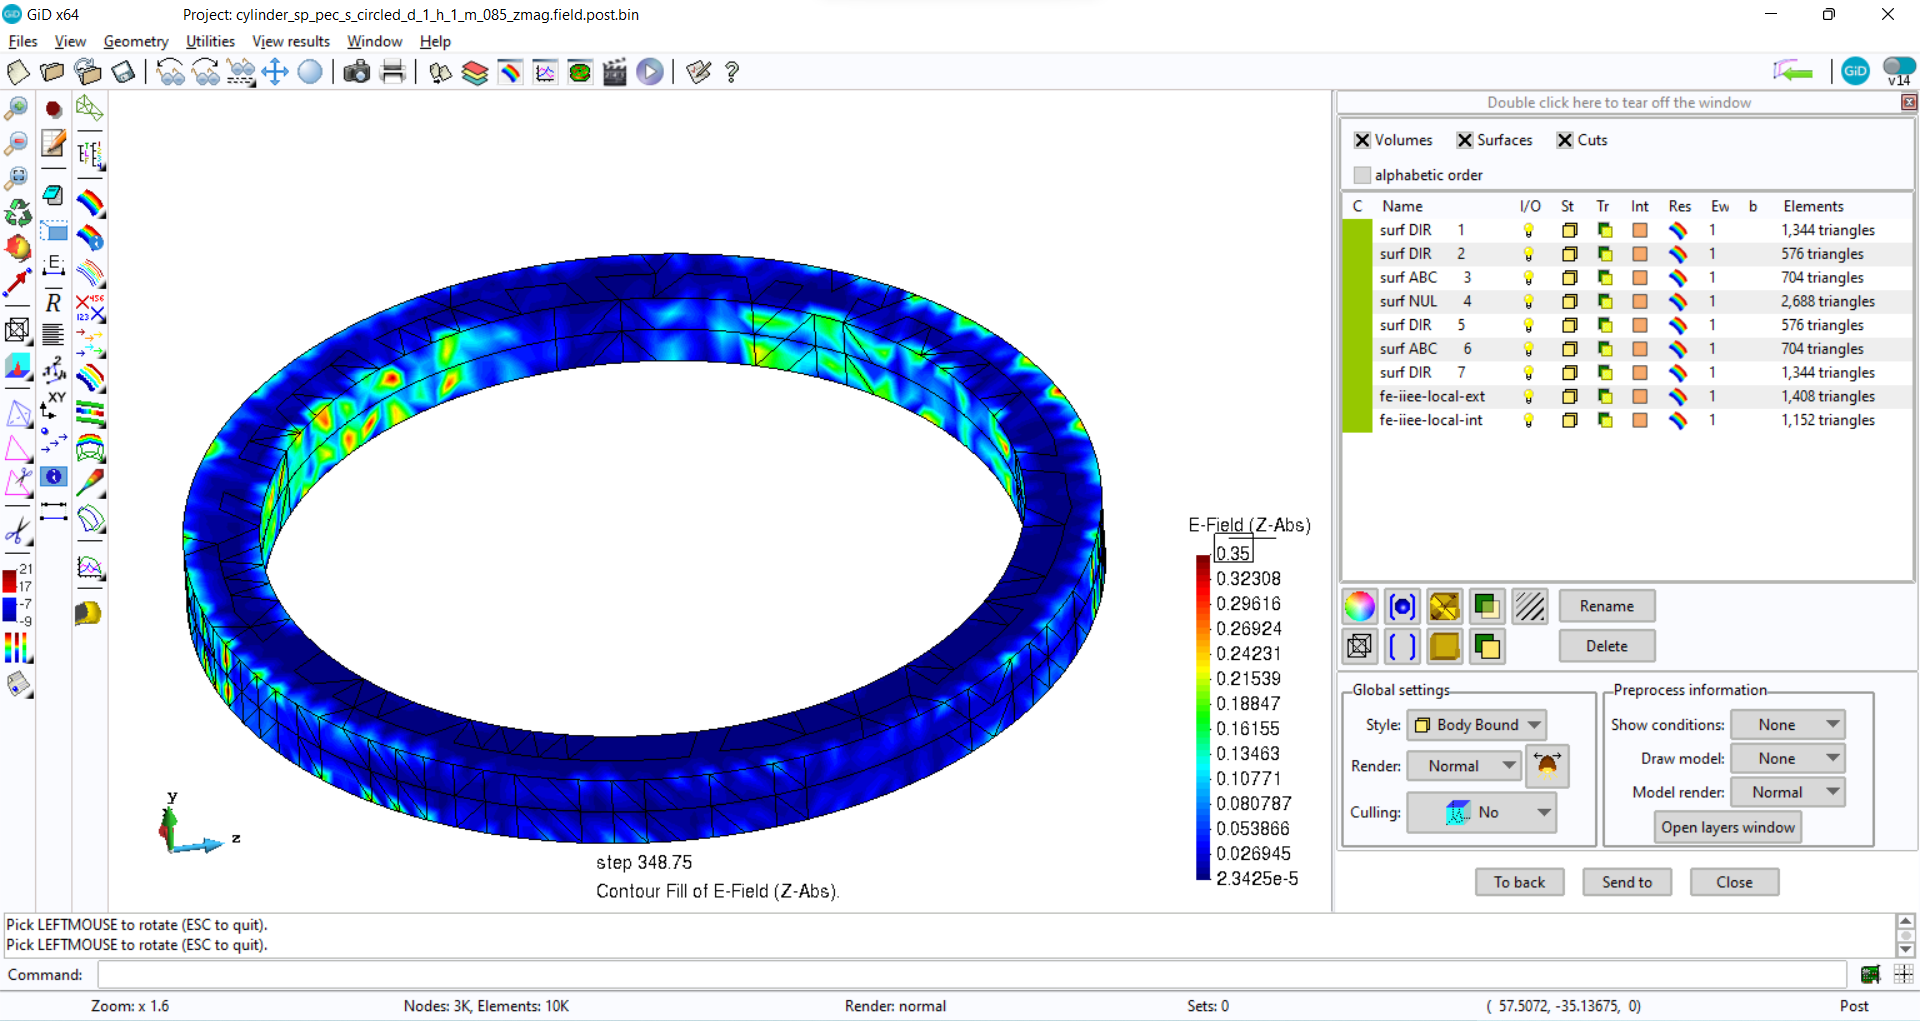
\includegraphics[width=\textwidth,clip=true,trim=70 0 350 140]
      {Ez_original} \\
      \footnotesize{$\abs{E_z}$ (default color scale)}
      \column{0.48\textwidth}\centering
      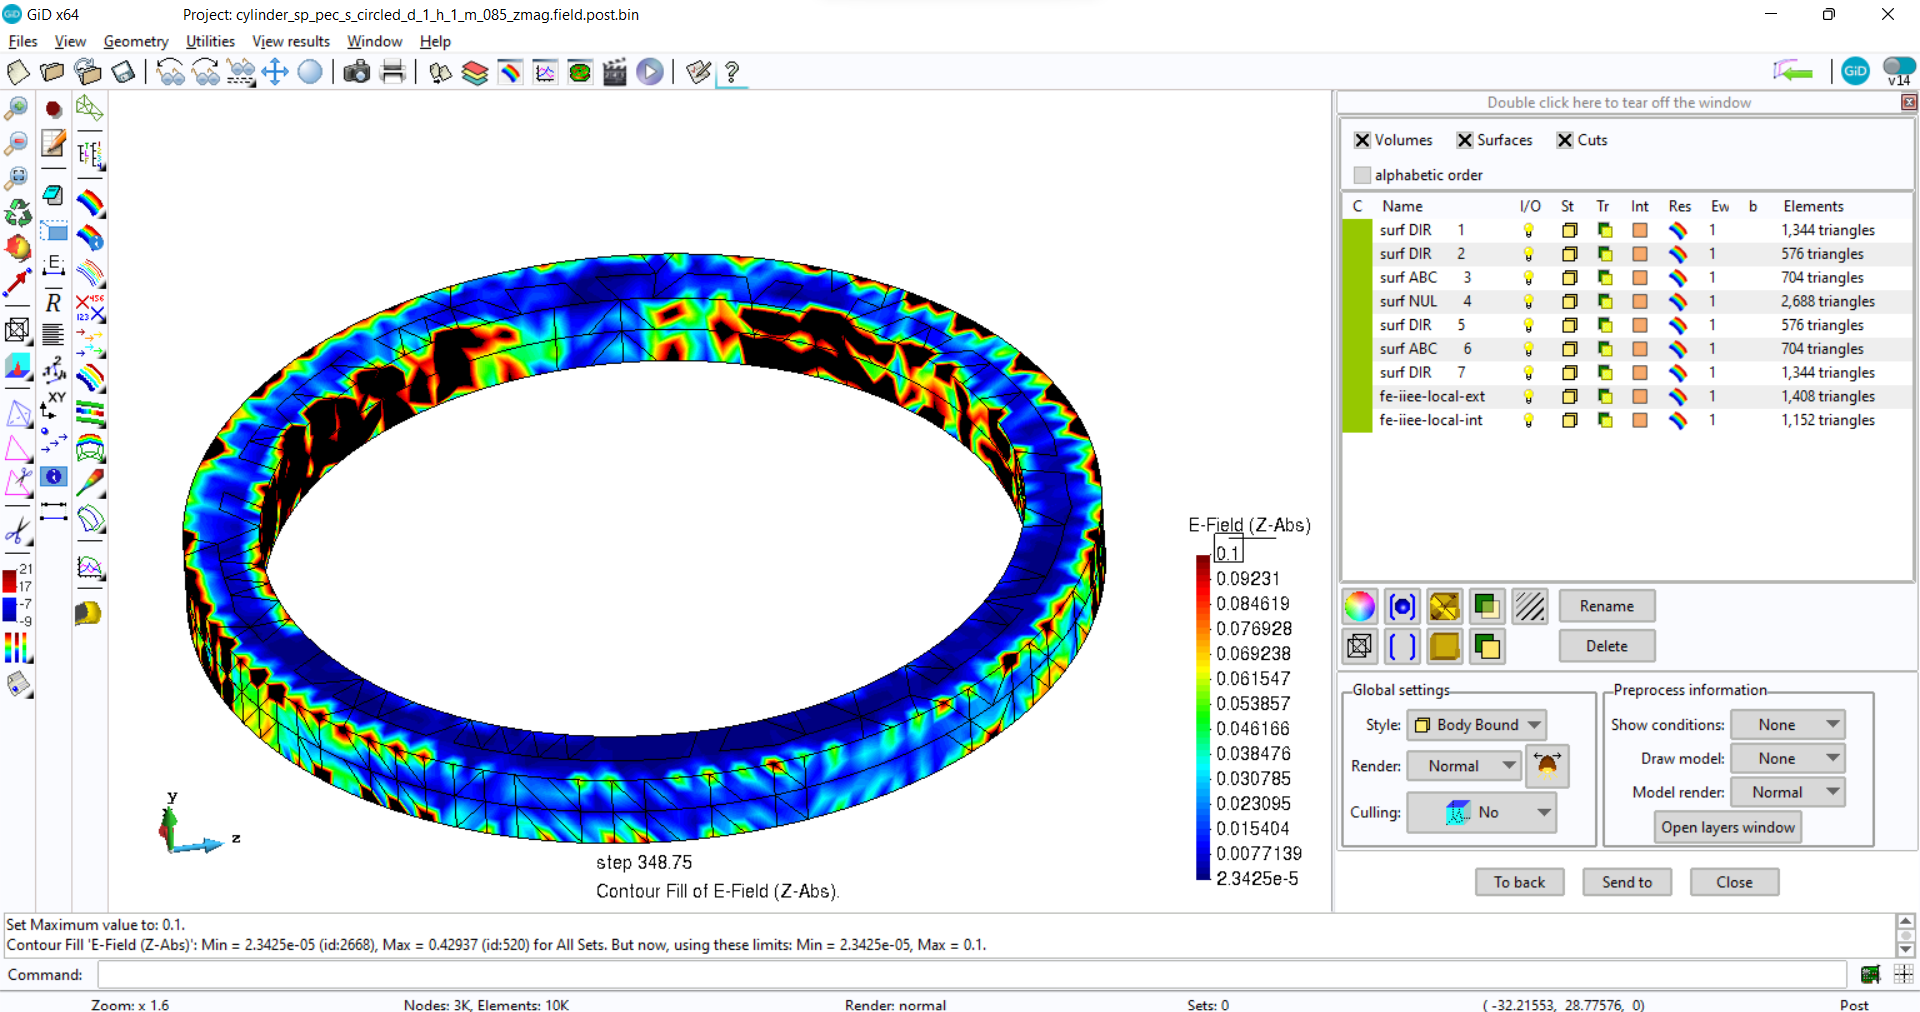
\includegraphics[width=\textwidth,clip=true,trim=70 0 350 140]
      {Ez_original_saturado_01} \\
      \footnotesize{$\abs{E_z}$ (saturated color scale)}
    \end{columns}
    

    \framebreak % %%%%%%%%%%%%%

  \item $E_y$ should be null on the cylinder ``sides'' (i.e., on the
    PEC cylinder)

    \vbss
   
    \begin{center}
     \begin{columns}%[T]
%      \column{0.48\textwidth}\centering
      % \includegraphics[width=\textwidth,clip=true,trim=70 0 350 140]
      % {Ey_original} \\
      % \footnotesize{$\abs{E_y}$ }
      \column{0.70\textwidth}\centering
      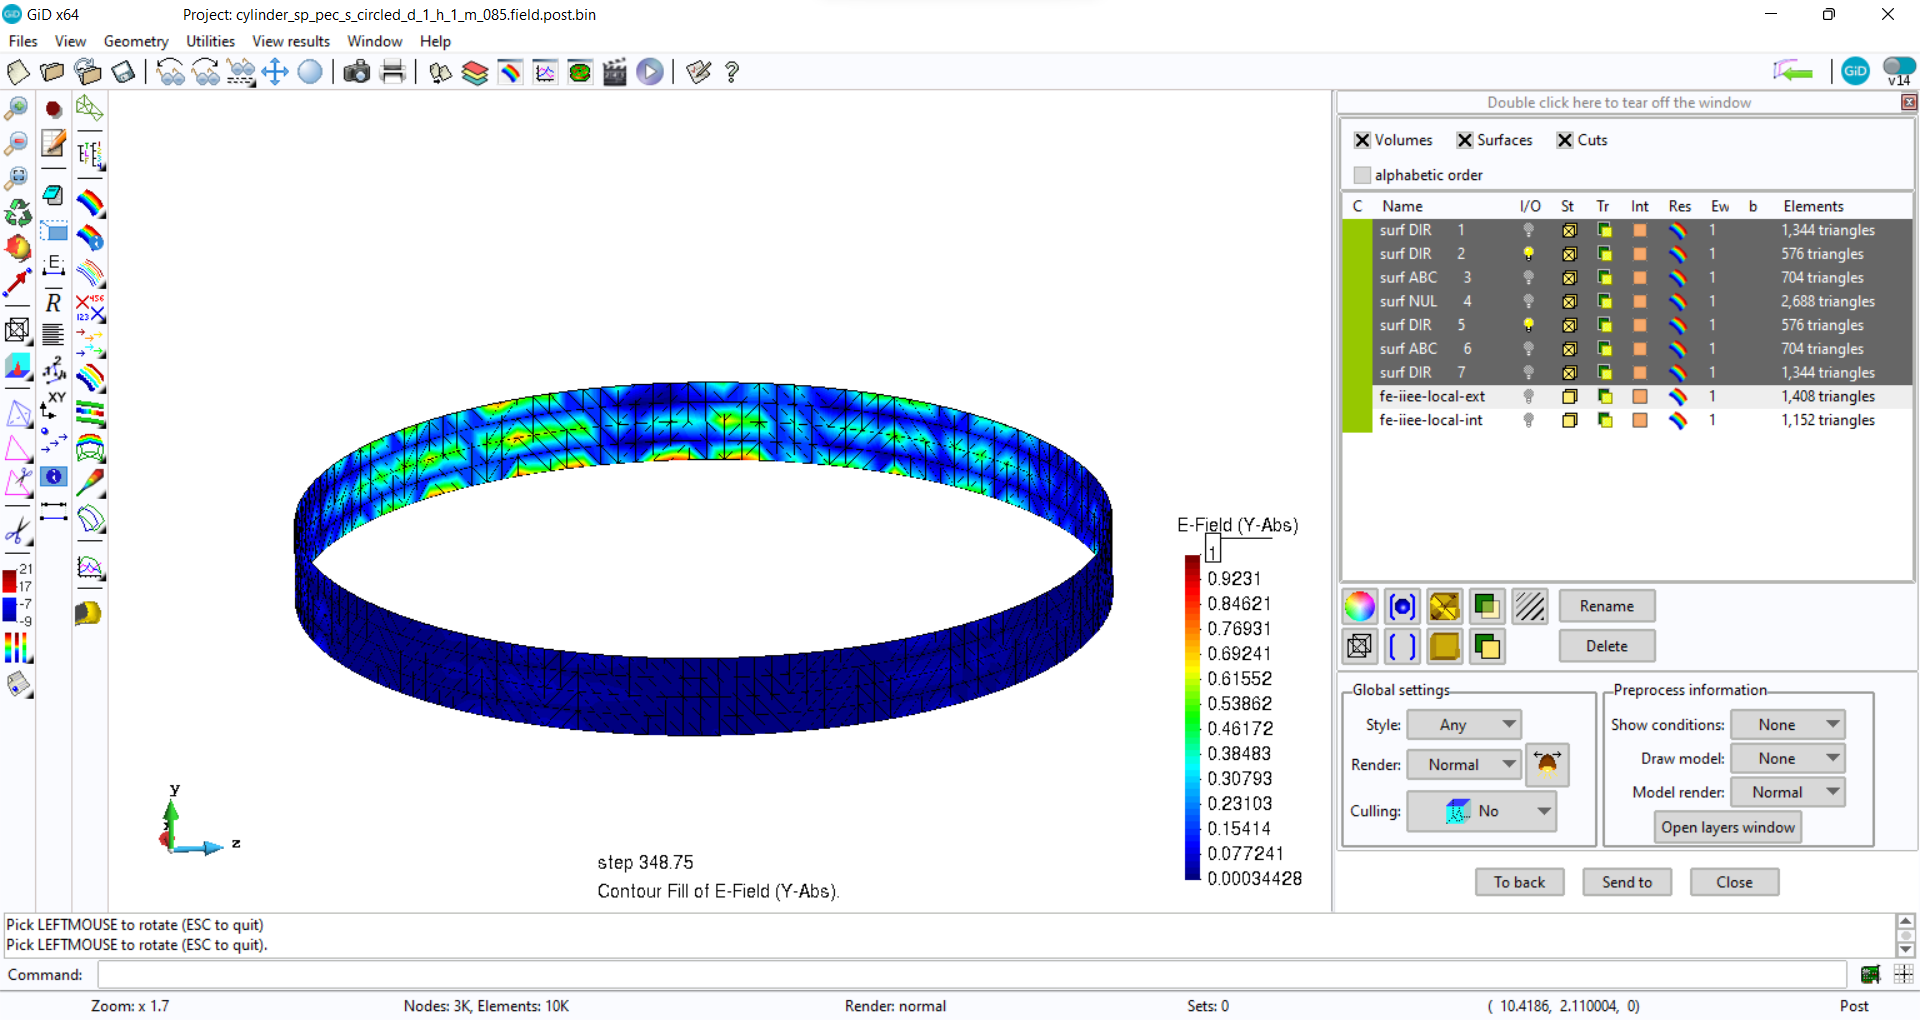
\includegraphics[width=\textwidth,clip=true,trim=70 0 350 140]
      {Ey_internal_cylinder} \\
      \footnotesize{$\abs{E_y}$ (only PEC cylinder surface shown)}
    \end{columns}
  \end{center}
  \end{itemize}
\end{frame}

% %%%%%%%%%%%%%%%%%%%%%%%%%%%%%%%%%%%%%%%%%%%%%%%%%%%%%%%%%%%%%%%

\begin{comment} % NO ES MUY CLARA LA CONCLUSION (por tema de como sale la Green3D o el campo  H) ASI QUE SE OMITEN

\begin{frame}[allowframebreaks]{Effect of Discretization}{Simple test
    changing frequency \alert{(note other electrical distances also
      change)}}


%    $300\,\text{MHz}$ \makebox[0pt][l]{20:}\hspace{2em}
    \raisebox{\baselineskip-\height}{
      \includegraphics[width=0.3\textwidth]
      {results/2D/20/300/\meshCCC{01}{1}{075}/E_S.pdf}
      \hspace{1cm}
      \includegraphics[width=0.3\textwidth]
      {results/2D/20/300/\meshCCC{01}{1}{075}/H_S.pdf}
    }

    
    \vbs

%    Lower frequency \makebox[0pt][l]{1:}\hspace{2em}
    \raisebox{\baselineskip-\height}{
      \includegraphics[width=0.3\textwidth]
      {results/2D/20/30/\meshCCC{01}{1}{075}/E_S.pdf}
      \hspace{1cm}
      \includegraphics[width=0.3\textwidth]
      {results/2D/20/30/\meshCCC{01}{1}{075}/H_S.pdf}
    }

  \end{frame}
  
\end{comment} % %%%%%%%%%%%
  
  % %%%%%%%%%%%%%%%%%%%%%%%%%%%%%%%%%%%%%%%%%%%%%%%%%%%%%%%%%%%%%%% 

\begin{comment} % NO ES MUY CLARA LA CONCLUSION (la quitamos)

\begin{frame}[allowframebreaks]{Effect of Distance $S'-S$}{Scattered near field}

    \begin{columns}
      \column{0.25\textwidth}
        \includegraphics[width=\linewidth]
        {results/2D/20/300/\meshCCC{01}{1}{075}/geometry.pdf}

        \includegraphics[width=\linewidth]
        {results/2D/20/300/\meshCCC{1}{1}{075}/geometry.pdf}
      \column{0.3\textwidth}
        
        \includegraphics[width=\linewidth]
        {results/2D/20/300/\meshCCC{01}{1}{075}/E_S.pdf}
        
        \includegraphics[width=\linewidth]
        {results/2D/20/300/\meshCCC{1}{1}{075}/E_S.pdf}

      
    \column{0.3\textwidth}
      \hfill\GreenT\hfill\mbox{}

        \includegraphics[width=\linewidth]
        {results/3D/20/300/\meshCCC{01}{1}{075}/E_S.pdf}
        
        \includegraphics[width=\linewidth]
        {results/3D/20/300/\meshCCC{1}{1}{075}/E_S.pdf}
        

    \end{columns}

    \begin{itemize}
    \item  {\GreenT} results always worse than {\GreenD}
    \item Difficult comparison ($S$ is not at the same electrical distance) 
    \end{itemize}
    
  \end{frame}

\end{comment}  % %%%%%

  % %%%%%%%%%%%%%%%%%%%%%%%%%%%%%%%%%%%%%%%%%%%%%%%%%%%%%%%%%%%%%%% 

\begin{comment} % Idem que anterior

  \begin{frame}[allowframebreaks]{Effect of Distance $S'-S$}{FEM solution}

    \begin{columns}
      \column{0.25\textwidth}

        \includegraphics[width=\linewidth]
        {results/2D/20/300/\meshCCC{01}{1}{075}/geometry.pdf}

        \includegraphics[width=\linewidth]
        {results/2D/20/300/\meshCCC{1}{1}{075}/geometry.pdf}
      \column{0.3\textwidth}
      \hfill\GreenD\hfill\mbox{}
        
        \includegraphics[width=\linewidth]
        {results/2D/20/300/\meshCCC{01}{1}{075}/E_Sp.pdf}
        
        \includegraphics[width=\linewidth]
        {results/2D/20/300/\meshCCC{1}{1}{075}/E_Sp.pdf}

      
    \column{0.3\textwidth}
      \hfill\GreenT\hfill\mbox{}

        \includegraphics[width=\linewidth]
        {results/3D/20/300/\meshCCC{01}{1}{075}/E_Sp.pdf}
        
        \includegraphics[width=\linewidth]
        {results/3D/20/300/\meshCCC{1}{1}{075}/E_Sp.pdf}
        

    \end{columns}

    \begin{itemize}
      \item The IIEE iterative method has low effect when $S-S'$ is larger.
    \end{itemize}
    
  \end{frame}
  
\end{comment}  % %%%%%
  
  % %%%%%%%%%%%%%%%%%%%%%%%%%%%%%%%%%%%%%%%%%%%%%%%%%%%%%%%%%%%%%%% 
  
\begin{frame}[allowframebreaks]{Effect of ``Thickness''}{Scattered
    near field ---\alert{Note error in figure captions: thickness is
      $0.05\,\lambda$ for the thin slice---}}
    
    \begin{columns}
      \column{0.25\textwidth}
        \includegraphics[width=\linewidth]
        {results/2D/20/300/\meshCCC{01}{1}{075}/geometry.pdf}

        \includegraphics[width=\linewidth]
        {results/2D/20/300/\meshCCC{01}{005}{075}/geometry.pdf}
      \column{0.3\textwidth}
      \hfill\GreenD\hfill\mbox{}
        
        \includegraphics[width=\linewidth]
        {results/2D/20/300/\meshCCC{01}{1}{075}/E_S.pdf}
        
        \includegraphics[width=\linewidth]
        {results/2D/20/300/\meshCCC{01}{005}{075}/E_S.pdf}

      
    \column{0.3\textwidth}
      \hfill\GreenT\hfill\mbox{}

        \includegraphics[width=\linewidth]
        {results/3D/20/300/\meshCCC{01}{1}{075}/E_S.pdf}
        
        \includegraphics[width=\linewidth]
        {results/3D/20/300/\meshCCC{01}{005}{075}/E_S.pdf}
        

    \end{columns}

  \end{frame}

  \begin{frame}[allowframebreaks]{Effect of ``Thickness''}{FEM solution
    ---\alert{Note error in figure captions: thickness is
      $0.05\,\lambda$ for the thin slice---}}
    
    \begin{columns}
      \column{0.25\textwidth}
        \includegraphics[width=\linewidth]
        {results/2D/20/300/\meshCCC{01}{1}{075}/geometry.pdf}

        \includegraphics[width=\linewidth]
        {results/2D/20/300/\meshCCC{01}{005}{075}/geometry.pdf}
      \column{0.3\textwidth}
      \hfill\GreenD\hfill\mbox{}
        
        \includegraphics[width=\linewidth]
        {results/2D/20/300/\meshCCC{01}{1}{075}/E_Sp.pdf}
        
        \includegraphics[width=\linewidth]
        {results/2D/20/300/\meshCCC{01}{005}{075}/E_Sp.pdf}

      
    \column{0.3\textwidth}
      \hfill\GreenT\hfill\mbox{}

        \includegraphics[width=\linewidth]
        {results/3D/20/300/\meshCCC{01}{1}{075}/E_Sp.pdf}
        
        \includegraphics[width=\linewidth]
        {results/3D/20/300/\meshCCC{01}{005}{075}/E_Sp.pdf}
        

    \end{columns}

    \framebreak 
    
    \begin{itemize}
    \item The thickness is the main factor for error with {\GreenT}
    \item {\GreenD} behaves great!
    \item Always lower error  with thin slices% (although convergence is slow)
    \end{itemize}
    
    
  \end{frame}

    

  % %%%%%%%%%%%%%%%%%%%%%%%%%%%%%%%%%%%%%%%%%%%%%%%%%%%%%%%%%%%%%%% 
  

  \begin{comment} %%%%%%%  POR HACER
    
  \begin{frame}[allowframebreaks]{Effect on Polarization Purity}

    \begin{itemize}
    \item With ``thickness'' \textbf{Usamos espesor gordo para que se
        note:} Por ejemplo, O bien
      \url{cylinder_sp_circled_s_circled_d_1_h_1_m_075} o bien
      \url{cylinder_sp_circled_s_circled_d_01_h_1_m_075} (no se en
      cual se notará mas según distancia S'-S, uhm.....)

      \vskip 1em
      
      \begin{columns}%[T]
      \column{0.48\textwidth}
      \FIGURA{\GreenT}
%      \includegraphics[width=\textwidth]{kk_iter1} \\
%      \footnotesize{kkkkk}
      \column{0.48\textwidth}
      \FIGURA{\GreenD}
%      \includegraphics[width=\textwidth]{kk_iter82} \\
      %\footnotesize{kkkk}
    \end{columns}
  \end{itemize}
    \begin{itemize}
    \item Conclusion 1
    \item \ldots
    \end{itemize}
    
  \end{frame}

  \end{comment} %%%%%%%%
  
  % %%%%%%%%%%%%%%%%%%%%%%%%%%%%%%%%%%%%%%%%%%%%%%%%%%%%%%%%%%%%%%% 
  
  \begin{frame}[allowframebreaks]{Other Effects (paranoic
      mode)}{Effect of $S'$ on PEC cylinder}

    \begin{columns}
    \column{0.25\textwidth}

        \includegraphics[width=\linewidth]
        {results/3D/20/300/\meshCCC{1}{1}{075}/geometry.pdf}
        
        \includegraphics[width=\linewidth]
        {results/3D/20/300/\meshPC{1}{1}{085}/geometry.pdf}
      \column{0.3\textwidth}

        \includegraphics[width=\linewidth]
        {results/2D/20/300/\meshCCC{1}{1}{075}/E_S.pdf}

        \includegraphics[width=\linewidth]
        {results/2D/20/300/\meshPC{1}{1}{085}/E_S.pdf}
      \column{0.3\textwidth}
        
        \includegraphics[width=\linewidth]
        {results/2D/20/300/\meshCCC{1}{1}{075}/H_S.pdf}
        
        \includegraphics[width=\linewidth]
        {results/2D/20/300/\meshPC{1}{1}{085}/H_S.pdf}

    \end{columns}
    
  \end{frame}


  % %%%%%%%%%%%%%%%%%%%%%%%%%%%%%%%%%%%%%%%%%%%%%%%%%%%%%%%%%%%%%%% 
  
  \begin{frame}[allowframebreaks]{Other Effects (paranoic
      mode)}{Effect of $S'$, $S$ Curved}
    
      \begin{columns}
    \column{0.25\textwidth}

        \includegraphics[width=\linewidth]
        {results/3D/20/300/\meshCCC{01}{1}{075}/geometry.pdf}
        
        \includegraphics[width=\linewidth]
        {results/3D/20/300/\meshCSS{01}{1}{075}/geometry.pdf}
      \column{0.3\textwidth}

        \includegraphics[width=\linewidth]
        {results/2D/20/300/\meshCCC{01}{1}{075}/E_S.pdf}

        \includegraphics[width=\linewidth]
        {results/2D/20/300/\meshCSS{01}{1}{075}/E_S.pdf}
      \column{0.3\textwidth}
        
        \includegraphics[width=\linewidth]
        {results/2D/20/300/\meshCCC{01}{1}{075}/H_S.pdf}
        
        \includegraphics[width=\linewidth]
        {results/2D/20/300/\meshCSS{01}{1}{075}/H_S.pdf}

      
        

    \end{columns}
    

    
  \end{frame}

% %%%%%%%%%%%%%%%%%%%%%%%%%%%%%%%%%%%%%%%%%%%%%%%%%%%%%%%%%%%%%%%

  \begin{frame}[allowframebreaks]{{\GreenT} vs {\GreenD}}{Conclusions}

    \begin{block}{Conclusions}
      \begin{itemize}
      \item {\GreenT} itself not valid for 2D Emulation
        \begin{itemize}
        \item FE-IIEE converges but
          \begin{itemize}
          \item Quality of solution far from great
          \item It may guide you to wrong solution
          \end{itemize}
        \end{itemize}
      \item Need to activate contributions of slice replicas along
        direction of cylinder (translation symmetry)
        \alert{\GreenTEw}, Section~\ref{sec:Ewald1D}
      \end{itemize}
    \end{block}
  
  \end{frame}

% %%%%%%%%%%%%%%%%%%%%%%%%%%%%%%%%%%%%%%%%%%%%%%%%%%%%%%%%%%%%%%%%%%%  

%\subsection{Further Numerical Results (using {\GreenD})}
  
  \begin{frame}[plain]
    From now on we only use {\GreenD}
    \begin{itemize}
    \item We check TE polarization for PEC cylinder
    \item We check for the dielectric coated  cylinder 
    \end{itemize}
  \end{frame}
  
% %%%%%%%%%%%%%%%%%%%%%%%%%%%%%%%%%%%%%%%%%%%%%%%%%%%%%%%%%%%%%%%
  \subsubsection{TE Polarization}
% %%%%%%%%%%%%%%%%%%%%%%%%%%%%%%%%%%%%%%%%%%%%%%%%%%%%%%%%%%%%%%%
  
  \begin{frame}[allowframebreaks]{Check TE polarization}{Comparison
      with TM results}
    
    \begin{columns}
      \column{0.5\linewidth}
      \includegraphics[width=\linewidth]{results/TE/geometry.pdf}
      
      \column{0.45\linewidth}
      \begin{itemize}
      \item
        Freq: 300\,MHz. ($\lambda=1\,$m)
      \item
        Thickness: 0.05\,m
      \end{itemize}
      
    \end{columns}
    
    \framebreak
    
    \begin{columns}
      \column{0.35\linewidth}
      \hfill TM incident field \hfill\mbox{}
      \vspace{1ex}
      \includegraphics[width=\linewidth]{results/TM/E_Sp.pdf}
      \includegraphics[width=\linewidth]{results/TM/E_S.pdf}
      
      \column{0.35\linewidth}
      \hfill TE incident field \hfill\mbox{}
      \vspace{1ex}
      \includegraphics[width=\linewidth]{results/TE/E_Sp.pdf}
      \includegraphics[width=\linewidth]{results/TE/E_S.pdf}
      
    \end{columns}
    
    \framebreak
    
    \begin{columns}
      \column{0.35\linewidth}
      \hfill TM incident field \hfill\mbox{}
      \vspace{1ex}
      \includegraphics[width=\linewidth]{results/TM/H_Sp.pdf}
      \includegraphics[width=\linewidth]{results/TM/H_S.pdf}
      
      \column{0.35\linewidth}
      \hfill TE incident field \hfill\mbox{}
      \vspace{1ex}
      \includegraphics[width=\linewidth]{results/TE/H_Sp.pdf}
      \includegraphics[width=\linewidth]{results/TE/H_S.pdf}
      
    \end{columns}
    
  \end{frame}

  % %%%%%%%%%%%%%%%%%%%%%%%%%%%%%%%%%%%%%%%%%%%%%%%%%%%%%%%%%%%%%%%%%%%%
  
% %%%%%%%%%%%%%%%%%%%%%%%%%%%%%%%%%%%%%%%%%%%%%%%%%%%%%%%%%%%%%%%
  \subsubsection{Dieletric Coated Cylinder (TM and TE)}
  % %%%%%%%%%%%%%%%%%%%%%%%%%%%%%%%%%%%%%%%%%%%%%%%%%%%%%%%%%%%%%%%
  
  \begin{frame}[allowframebreaks]{Dielectric Coated Cylinders}{Comparison with the analytical solution }

    
    \begin{columns}
      \column{0.5\linewidth}
      \includegraphics[width=\linewidth]{results/TMc4/geometry.pdf}
      
      \column{0.45\linewidth}
      \begin{itemize}
      \item
        Freq: 300\,MHz. ($\lambda=1\,$m)
      \item
        Thickness: 0.05\,m
      \item
        Dielectric substrate between $S$ and $S'$ with relative permittivity 
        $\varepsilon_r$.
      \end{itemize}
    \end{columns}

    \framebreak
        
    \hfill TM incident field $\varepsilon_r=1$ \hfill\mbox{}

    \begin{columns}
      \column{0.35\linewidth}
      \includegraphics[width=\linewidth]{results/TM/E_Sp.pdf}

      \includegraphics[width=\linewidth]{results/TM/E_S.pdf}
      
      \column{0.35\linewidth}
      \includegraphics[width=\linewidth]{results/TM/H_Sp.pdf}

      \includegraphics[width=\linewidth]{results/TM/H_S.pdf}
      
    \end{columns}
    
    \framebreak
        
    \hfill TM incident field $\varepsilon_r=4$ \hfill\mbox{}

    \begin{columns}
      \column{0.35\linewidth}
      \includegraphics[width=\linewidth]{results/TMc4/E_Sp.pdf}

      \includegraphics[width=\linewidth]{results/TMc4/E_S.pdf}
      
      \column{0.35\linewidth}
      \includegraphics[width=\linewidth]{results/TMc4/H_Sp.pdf}

      \includegraphics[width=\linewidth]{results/TMc4/H_S.pdf}
      
    \end{columns}
    
    \framebreak

    \hfill TE incident field $\varepsilon_r=1$ \hfill\mbox{}
    
    \begin{columns}
      \column{0.35\linewidth}
      \includegraphics[width=\linewidth]{results/TE/E_Sp.pdf}

      \includegraphics[width=\linewidth]{results/TE/E_S.pdf}
      
      \column{0.35\linewidth}
      \includegraphics[width=\linewidth]{results/TE/H_Sp.pdf}

      \includegraphics[width=\linewidth]{results/TE/H_S.pdf}
      
    \end{columns}

    \framebreak

    \hfill TE incident field $\varepsilon_r=1.5$ \hfill\mbox{}
    
    \begin{columns}
      \column{0.35\linewidth}
      \includegraphics[width=\linewidth]{results/TEc15/E_Sp.pdf}

      \includegraphics[width=\linewidth]{results/TEc15/E_S.pdf}
      
      \column{0.35\linewidth}
      \includegraphics[width=\linewidth]{results/TEc15/H_Sp.pdf}

      \includegraphics[width=\linewidth]{results/TEc15/H_S.pdf}
      
    \end{columns}
    




  \end{frame}

  
  % %%%%%%%%%%%%%%%%%%%%%%%%%%%%%%%%%%%%%%%%%%%%%%%%%%%%%%%%%%%%%%%
